%%%%%%%%%%%%%%%%%%%%%%%%%%%%%%%%%%%%%%%%%%%%%%%%%%%%%%%%%%%%%%%%%%%%%%%%%%%%%%%%%%
\begin{frame}[fragile]\frametitle{}

\begin{center}
{\Large Clustering}
\end{center}
\end{frame}
%%%%%%%%%%%%%%%%%%%%%%%%%%%%%%%%%%%%%%%%%%%%%%%%%%%%%%%%%%%%%%%%%%%%%%%%%%%%%%%%%%
\begin{frame}[fragile]
  \frametitle{Text Clustering}
\begin{itemize}
\item Finds overall similarities among groups of documents
\item Finds overall similarities among groups of tokens (words, adjectives)
\item Goal is to place similar objects in the same groups and to assign dissimilar objects to different groups
\end{itemize}
\end{frame}

%%%%%%%%%%%%%%%%%%%%%%%%%%%%%%%%%%%%%%%%%%%%%%%%%%%%%%%%%%%%%%%%%%%%%%%%%%%%%%%%%%
\begin{frame}[fragile]
  \frametitle{Document clustering}
\begin{center}
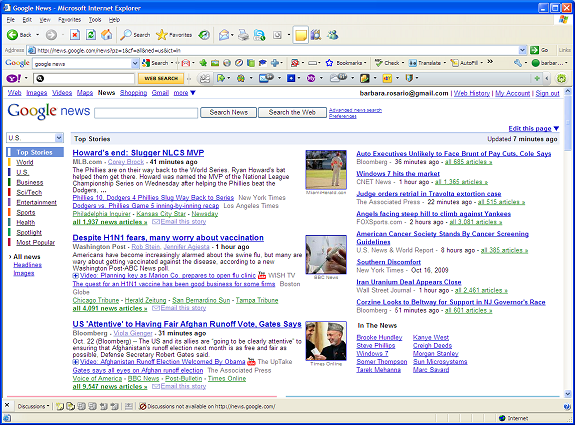
\includegraphics[width=0.8\linewidth,keepaspectratio]{class18}
\end{center}
\end{frame}

%%%%%%%%%%%%%%%%%%%%%%%%%%%%%%%%%%%%%%%%%%%%%%%%%%%%%%%%%%%%%%%%%%%%%%%%%%%%%%%%%%
\begin{frame}[fragile]
  \frametitle{Unsupervised Classification}
\begin{itemize}
\item Classification when labeled data is not available 
\item Results of clustering depends only on the natural division in the data, not on any pre-existing categorization scheme
\item Hard/Soft Clustering
\item Flat/hierarchical clustering

\item Similarity measures
\end{itemize}
\end{frame}

%%%%%%%%%%%%%%%%%%%%%%%%%%%%%%%%%%%%%%%%%%%%%%%%%%%%%%%%%%%%%%%%%%%%%%%%%%%%%%%%%%
\begin{frame}[fragile]
  \frametitle{Hard/soft Clustering}
\begin{center}
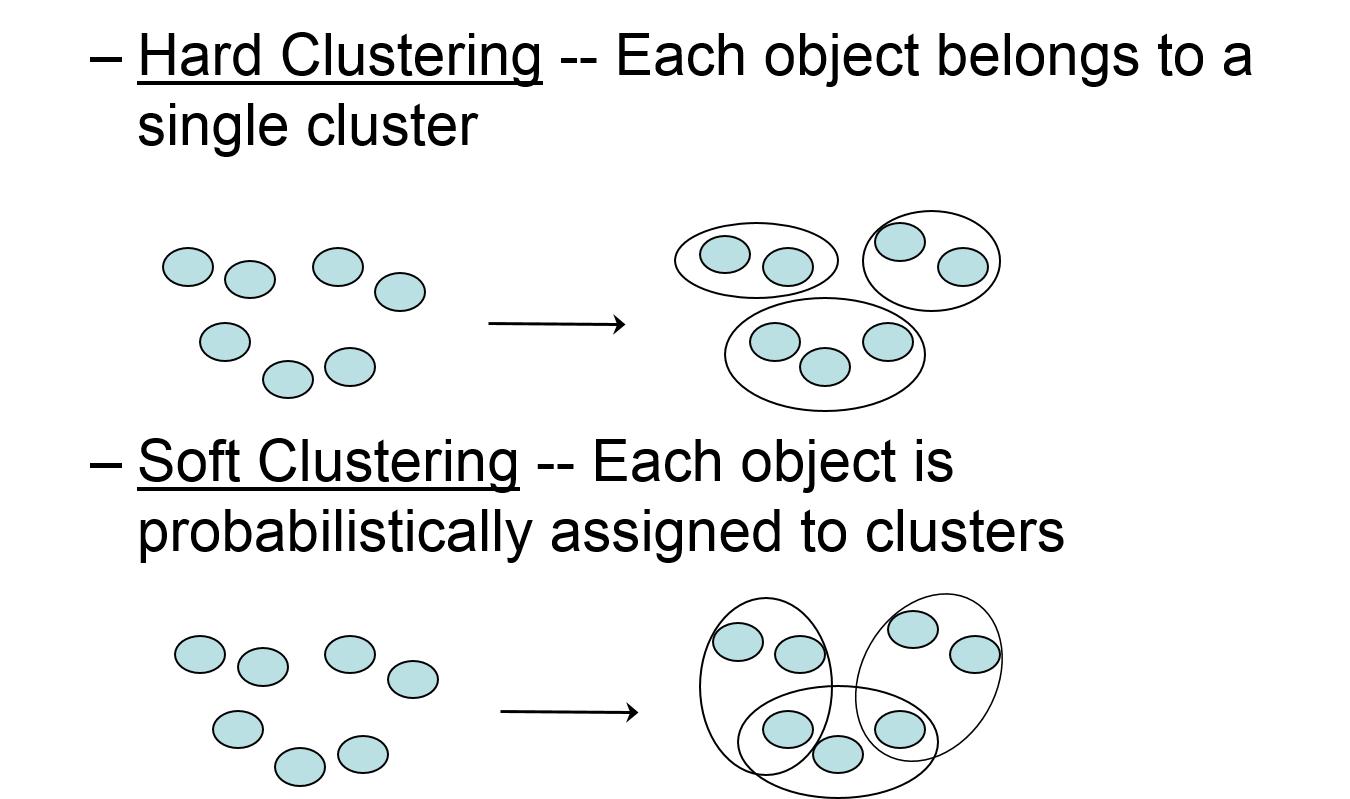
\includegraphics[width=\linewidth,keepaspectratio]{class19}
\end{center}
\end{frame}


%%%%%%%%%%%%%%%%%%%%%%%%%%%%%%%%%%%%%%%%%%%%%%%%%%%%%%%%%%%%%%%%%%%%%%%%%%%%%%%%%%
\begin{frame}[fragile]
  \frametitle{Hard/soft Clustering}
\begin{center}
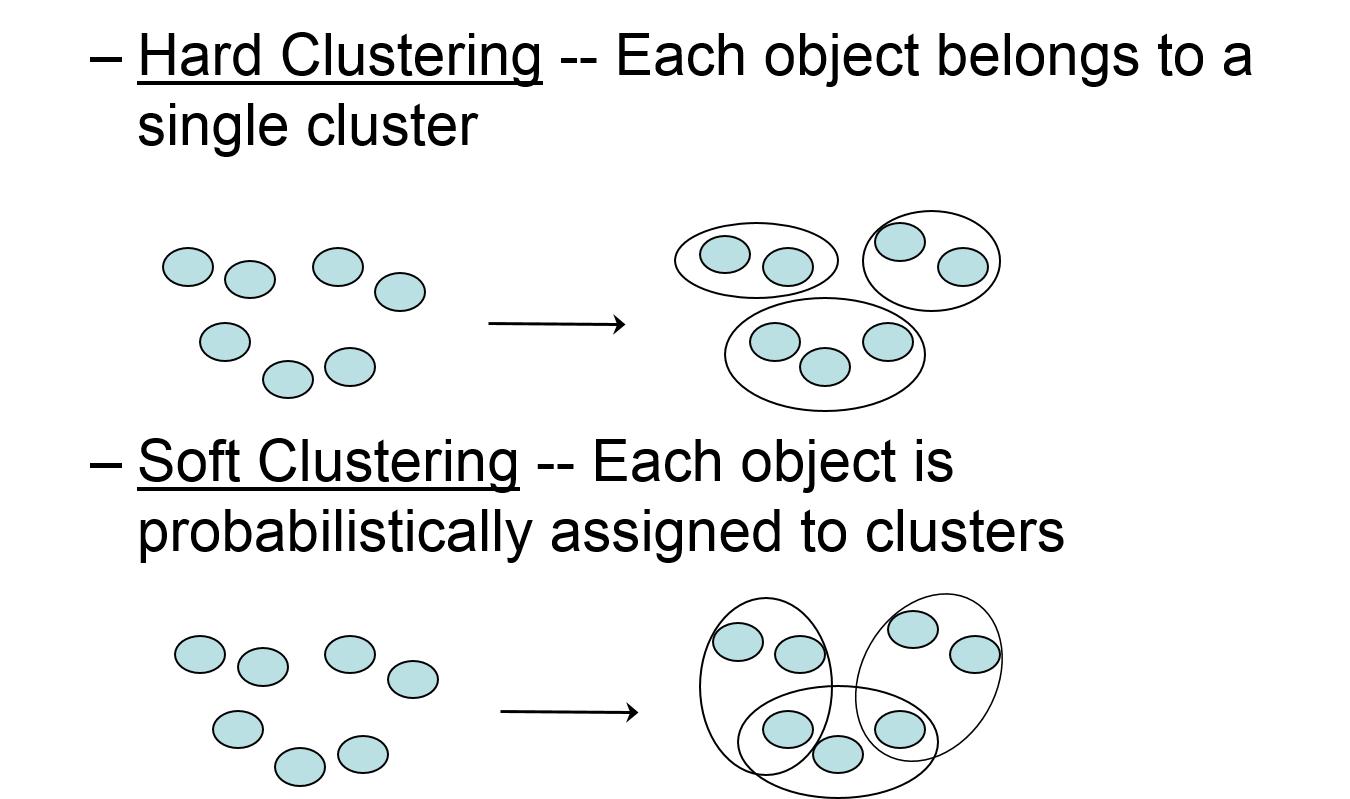
\includegraphics[width=\linewidth,keepaspectratio]{class19}
\end{center}
\end{frame}


%%%%%%%%%%%%%%%%%%%%%%%%%%%%%%%%%%%%%%%%%%%%%%%%%%%%%%%%%%%%%%%%%%%%%%%%%%%%%%%%%%
\begin{frame}[fragile]
  \frametitle{Flat Vs. Hierarchical }
\begin{itemize}
\item Flat clustering creates a flat set of clusters without any explicit structure that would relate clusters to each other
\item Hierarchical clustering produces a hierarchy of nodes	
\item Leaves are the single objects  of the clustered set
\item Node represents the cluster that contains all the nodes of its descendant
\end{itemize}
\end{frame}

%%%%%%%%%%%%%%%%%%%%%%%%%%%%%%%%%%%%%%%%%%%%%%%%%%%%%%%%%%%%%%%%%%%%%%%%%%%%%%%%%%
\begin{frame}[fragile]
  \frametitle{Similarity}
\begin{itemize}
\item Vector-space representation and similarity computation
\item Select important distributional properties of a word
\item Create a vector of length n for each word to be classified
\item Viewing the n-dimensional vector as a point in an n-dimensional space, cluster points that are near one another

\end{itemize}
\end{frame}

%%%%%%%%%%%%%%%%%%%%%%%%%%%%%%%%%%%%%%%%%%%%%%%%%%%%%%%%%%%%%%%%%%%%%%%%%%%%%%%%%%
\begin{frame}[fragile]
  \frametitle{Euclidean Similarity}
\begin{center}
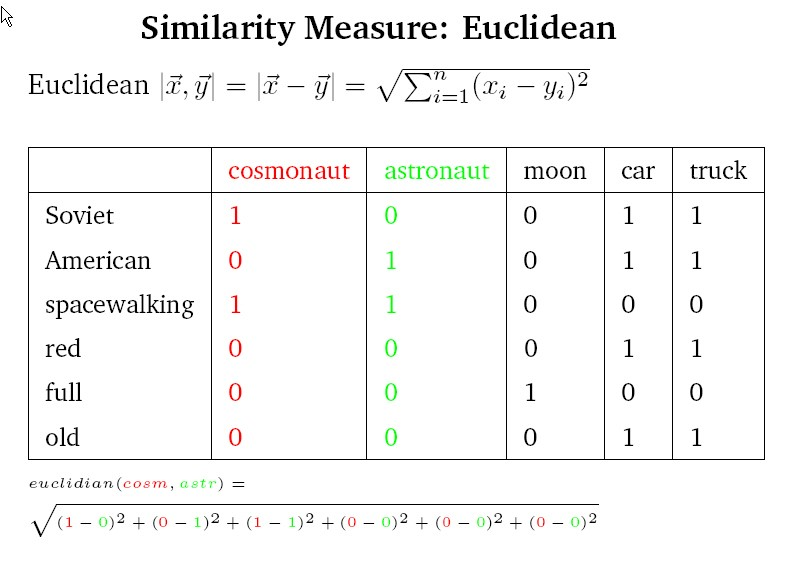
\includegraphics[width=\linewidth,keepaspectratio]{class20}
\end{center}
\end{frame}

%%%%%%%%%%%%%%%%%%%%%%%%%%%%%%%%%%%%%%%%%%%%%%%%%%%%%%%%%%%%%%%%%%%%%%%%%%%%%%%%%%
\begin{frame}[fragile]
  \frametitle{Cosine Similarity}
\begin{center}
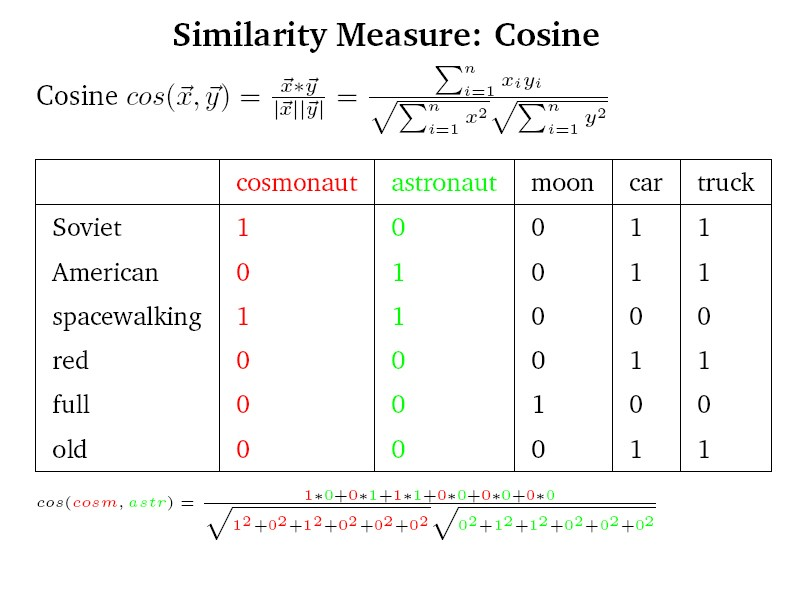
\includegraphics[width=\linewidth,keepaspectratio]{class21}
\end{center}
\end{frame}

%%%%%%%%%%%%%%%%%%%%%%%%%%%%%%%%%%%%%%%%%%%%%%%%%%%%%%%%%%%%%%%%%%%%%%%%%%%%%%%%%%
\begin{frame}[fragile]
  \frametitle{Flat Clustering: K-means}
\begin{itemize}
\item K-means is the most important flat clustering algorithm. 
\item Objective is to minimize the average squared Euclidean distance of documents from their cluster centers
\item Steps:
\begin{itemize}
\item Decide on a pair-wise similarity measure
\item Compute K centroids
\item Assign each document to nearest center, forming new clusters
\item  Unless terminate condition, previous 1-2
\end{itemize}
\end{itemize}
\end{frame}

%%%%%%%%%%%%%%%%%%%%%%%%%%%%%%%%%%%%%%%%%%%%%%%%%%%%%%%%%%%%%%%%%%%%%%%%%%%%%%%%%%
\begin{frame}[fragile]
  \frametitle{How to evaluate clusters?}
\begin{itemize}
\item In practice, it's hard to do
\item Different algorithms' results look good and bad in different ways
\item It's difficult to distinguish their outcomes
\item In theory, define an evaluation function
\item Typically choose something easy to measure (e.g., the sum of the average distance in each class)
\end{itemize}
\end{frame}